\documentclass[]{IEEEtran}

\title{Modeling and Synthesis of a Single-Precision Floating-point IEEE 754 Multiplier}
\author{Fabio Chiarani - VR445566}

\usepackage{graphicx}
\usepackage[british]{babel}
\usepackage{multicol}

\usepackage{tikz}
\usetikzlibrary{arrows,automata, positioning}
\usepackage[latin1]{inputenc}

\usepackage{forest}
\usepackage{xcolor}
\usepackage{listings}
\usepackage{booktabs}
\usepackage{hyperref}


\begin{document}
	\maketitle
	
	\begin{abstract}
		The following document shows how two parallel and equal IEEE 754 single precision floating-point multipliers have been realized through the modelling and synthesis by two HDL languages (SystemVerilog and VHDL). The goal is to use one toplevel that controls both multipliers, thus managing a hand-shake and serializing the output when is done. The synthesis produced, will be compared with a synthesis of a C floating point using the High Level Synthesis.
	\end{abstract}
	
	
	\section{Introduction}
	
	The project want to model a toplevel that controls two multipliers that perform multiplication according to the IEEE754 standard. The toplevel must be synthetized for an FPGA with only 125 ports (I/O) available. It is therefore necessary that the toplevel manages and serializes the inputs and outputs. 
	
	The toplevel is tested through a testbench, which reads inputs from a file. After that will be synthetized and its maximum clock speed will be evaluated (with other timings and area reports).
	
	The toplevel, written in VHDL and Verilog, it has also written in SystemC, to view how it is possible to describe and model a program in different levels of abstraction. Then, the timings report obtained will be compared with the C algorithm description of the IEEE 754 multiplication timing report retrived from the High Level Synthesis.
	
		The Verilog toplevel is synthetized with $444$ LUT, $395$ FF, $1$ BUFG, a minimum clock of $9ns$ and a power stimation of $0.112W$ with $26.4$ celsius degree for the junction temperature.
	\\
	
	The \hyperref[sec:Background]{'Background'} section gives some information about HDL languages and the IEEE 754 standard.
	Inside \hyperref[sec:impl]{'Implementation'} is described how the project is made: from the creation of the EFSM to the High Level Synthesis of the C algorithm. 
	
	Section \hyperref[sec:archvhdl]{'Architecture of VHD/Verilog RTL'} show the hardware architecture, interface and EFSM, while the section \hyperref[sec:archsystemc]{'Architecture of SystemC RTL'} show the architecture and the project structure for the SystemC modelling.
	

	After that, the \hyperref[sec:rtlsim]{'RTL Simulation'} section report the simulation phase of the Verilog and SystemC multipliers. Then the synthesis process are described inside the \hyperref[sec:rtlsim]{'Synthesis'} section, followed by the 
	\hyperref[sec:impl]{'Implementation'} section that provides the timing and area reports. Finally, the data obtained by the C HLS is reported on the \hyperref[sec:hls]{'HLS'} section.
	

	\section{Background}
	\label{sec:Background}
	
	HDL is a specialized language used to describe the structure and behavior of electronic circuits, and most commonly, digital logic circuits. It enables a formal description of an electronic circuit that allows for the automated analysis and simulation of an electronic circuit. It also allows for the synthesis of a HDL description into a netlist, which can then be placed and routed to produce the set of masks used to create an integrated circuit. ~\cite{hdlwikipedia}
	
	The two IEEE standard in common use are Verilog and VHDL. This two languages are common on RLT describing level. The High Level Synthesis ($HLS$)  ~\cite{hls} is another choice that can be adopted to execute the automatic translation and synthesis of an algorithmic description written in C, C++ or SystemC.
	
	In hardware design there are different levels of abstraction, on which different languages can operate, each with its own advantages and disadvantages. Generically, is possible to describe the system on RLT level with VHDL or Verilog, then making the synthesis to have the gate level. Another way is to make the HLS from a behavioral description by a SystemC, C or C++ description. A possible flow is shown below:
	
	\begin{center}
		
		
		\tikzset{every picture/.style={line width=0.75pt}} %set default line width to 0.75pt        
		
		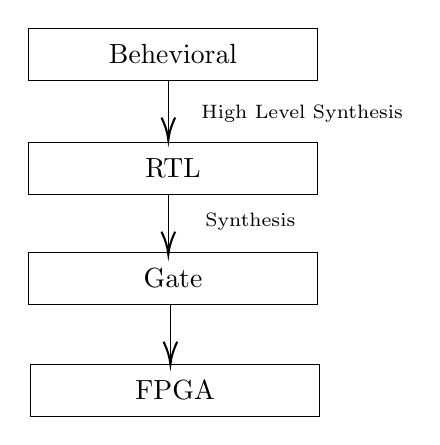
\begin{tikzpicture}[x=0.75pt,y=0.75pt,yscale=-1,xscale=1]
		%uncomment if require: \path (0,207); %set diagram left start at 0, and has height of 207
		
		%Shape: Rectangle [id:dp852547878604737] 
		\draw   (10,6) -- (149.5,6) -- (149.5,31) -- (10,31) -- cycle ;
		%Shape: Rectangle [id:dp05901974379796271] 
		\draw   (10,61) -- (149.5,61) -- (149.5,86) -- (10,86) -- cycle ;
		%Shape: Rectangle [id:dp9240181080439417] 
		\draw   (10,114) -- (149.5,114) -- (149.5,139) -- (10,139) -- cycle ;
		%Shape: Rectangle [id:dp49188121194132917] 
		\draw   (11,168) -- (150.5,168) -- (150.5,193) -- (11,193) -- cycle ;
		%Straight Lines [id:da0890493002877224] 
		\draw    (77.5,31) -- (77.5,57.97) ;
		\draw [shift={(77.5,59.97)}, rotate = 270] [color={rgb, 255:red, 0; green, 0; blue, 0 }  ][line width=0.75]    (10.93,-3.29) .. controls (6.95,-1.4) and (3.31,-0.3) .. (0,0) .. controls (3.31,0.3) and (6.95,1.4) .. (10.93,3.29)   ;
		
		%Straight Lines [id:da08058959401931964] 
		\draw    (77.5,86) -- (77.5,112.97) ;
		\draw [shift={(77.5,114.97)}, rotate = 270] [color={rgb, 255:red, 0; green, 0; blue, 0 }  ][line width=0.75]    (10.93,-3.29) .. controls (6.95,-1.4) and (3.31,-0.3) .. (0,0) .. controls (3.31,0.3) and (6.95,1.4) .. (10.93,3.29)   ;
		
		%Straight Lines [id:da9514171477188609] 
		\draw    (78.5,139) -- (78.5,165.97) ;
		\draw [shift={(78.5,167.97)}, rotate = 270] [color={rgb, 255:red, 0; green, 0; blue, 0 }  ][line width=0.75]    (10.93,-3.29) .. controls (6.95,-1.4) and (3.31,-0.3) .. (0,0) .. controls (3.31,0.3) and (6.95,1.4) .. (10.93,3.29)   ;
		
		
		% Text Node
		\draw (79.75,18.5) node   [align=left] {Behevioral};
		% Text Node
		\draw (79.75,73.5) node   [align=left] {RTL};
		% Text Node
		\draw (79.75,126.5) node   [align=left] {Gate};
		% Text Node
		\draw (80.75,180.5) node   [align=left] {FPGA};
		% Text Node
		\draw (142,47) node  [font=\scriptsize] [align=left] {High Level Synthesis};
		% Text Node
		\draw (117,99) node  [font=\scriptsize] [align=left] {Synthesis};
		
		
		\end{tikzpicture}
		
	\end{center}
	
	Through tools such as Vivado ~\cite{vivado}, is possible to set some constraints that must be respected (e.g. clock requency) by the design. In this way the tool shows if the design respects these constraints, proceeding with the implementation, or it is necessary to refine the system.
	After the synthesis and implementation is possible to view the timing reports, latency and area of the generated model.
	\\
	
	In IEEE 754-2008 the 32-bit base 2 format is officially referred to as binary32. It was called single in IEEE 754-1985. The IEEE 754 standard specifies a binary32 as having 1-bit sign, 8-bits for exponent and 24-bits for significand precision. The IEEE 754 provides a A full description of the IEEE754 standard can be viewed on Wikipedia ~\cite{wikiieee754}. The IEEE 754 arithmetic (used in this project) can be viewed on Wikipedia ~\cite{wikiarich754}.
	
	\section{Implementation}
	\label{sec:impl}
		After analyzing the required specifications, it was decided to design the system through an EFSM. This type of development has been useful in understanding well the system flow and the calculations that must be performed. In a second phase of review, having an EFSM, makes possible to do some improvements e.g. minimizing the number of states and/or transactions.
	
	After the EFSM definition, the RTL level components were developed first: the VHDL multiplier was created, tested through a minimal testbench to verify its correctness and, after that, the specular multiplier was written in Verilog.
	
	The toplevel and main testbench of the project is written in Verilog. It has been chosen to create a testbench that sends the same data to both modules to verify its correctness at the same time. The data is loaded from a file.
	\\
	
	Then I moved to the creation of the RTL part (composed by the same components and EFSM) in SystemC. The SystemC RTL project is however written with a synthesizable grammar. The testbench, having the same EFSM as the project written in VHDL, and properly tested, was not written by inputting values from files, but only 15-20 cases were tested to verify its correctness.
	
	The last part of the project, the HLS, was performed from an algorithmic description of the floating point multiplication in C++.
	The project architecture can be seen divided into two parts: the testbench (\textit{tb}) and the toplevel (\textit{tl}). The same architecture is used within the RTL description in Verilog/VHDL and SystemC.
	The architecture will be described according to a bottom-up approach, from the internal IEEE754 component to the toplevel:
	
	\section{Architecture of VHD/Verilog RTL}
	\label{sec:archvhdl}
	This section shows the architecture and the hardware description.
	
	\subsection{IEEE754 Multiplier}
	The multiplier component perform the floating point single-precision multiplication according to the IEE754 standard. The assumption is that the imputs are already normalized values, otherwise the multipler returns all $res$ signal with all zeros.
		
	\subsubsection{Component Interface}
	The Figure~\ref{fig:mul_ieee_754_schema} shows the module interfaces. It have 5 inputs and 2 outputs:
	\begin{itemize}
		\item [-] $[op1]$ is the first number of the multiplication.
		\item [-] $[op2]$ is the second number of the multiplication.
		\item [-] $[inrdy] $ tell to the module when the input are ready to compute the multiplication.
		\item [-] $[reset]$ reset the module.
		\item [-] $[clk]$ clock signal.
		\item [-] $[res]$ result of multiplication.
		\item [-] $[resrdy]$ tells when the result ($res$) is ready.
	\end{itemize}
	
	Inside on the VHDL module, on the architecture, there are 9 signals to handle data during the multiplication. Instead, on the Verilog module there are 9 registers. The data types are $STD\_LOGIC$, choosed for the possibility to make a better testbench simulation with the type propreties. 
	\\
	
	Both VHDL and Verilog module are modeled with 2 processes: the fsm and the datapath. The fsm manages the current and the next state; the datapath calculates. The datapath is driven by the clock and the fsm by the state signal.
	The EFSM of the multiplier is show below.
	
	\subsubsection{Component EFSM}
	The multiplier EFSM showed in Figure~\ref{fig:efsm_mul} describes the multiplication algorithm.
	Is composed of 21 states, handles infinite, zero and NaN cases and the rounding algorithm according to the IEEE754 standard.
	
	Short description of the sates:
	\begin{itemize}
		\item [-] [$s_0$] Initial and reset state.
		\item [-] [$s_1$] The machine stays here until input data are ready.
		\item [-] [$s_2$] Dispatch the input type.
		\item [-] [$Inf$] Handle infinity input value.
		\item [-] [$Zero$] Handle zero input value.
		\item [-] [$NaN$] Handle NaN input value.
		\item [-] [$err$] Return all zeros as output for show the invalid input error.
		\item [-] [$s_6$] Dispatch from normalized and denormalized input (if denormalized move to err).
		\item [-] [$s_10$] Make the multiplication.
		\item [-] [$s_11$] Normalize the value.
		\item [-] [$s_12$] Check for overflow or underflow.
		\item [-] [$s_13$] Handle overflow case.
		\item [-] [$s_14$] Handle underflow and correct case.
		\item [-] [$norm$] Reached when got a normalized input.
		\item [-] [$denorm$] Reached when got a denormalized input.
		\item [-] [$s_15$] Save on result the new exponent.
		\item [-] [$s_16$] Dispatch if need a shift.
		\item [-] [$s_17$] Save on result the mantissa.
		\item [-] [$s_18$] Shift operation.
		\item [-] [$s_19$] Save on result the exponent.
		\item [-] [$out$] Output the res value and return to the inital state.
	\end{itemize}

	\subsection{TopLevel}
	The toplevel, written in Verilog, has the task of instantiating a VHDL and Verilog multiplier, for performing the multiplication.
	
	\subsubsection{Component Interface}
	Since the FPGA has 125 ports, and the inputs are composed by 32 bit, it was not possible for the top level to accept all the 4 inputs at the same time. The toplevel interface schema is shown on Figure~\ref{fig:tl}, and the architectural choices were made as follows:
	\begin{itemize}
		\item [-] The toplevel accepts in input two values at a time. Inputs can be sent to all the two internal machine (Verlog and VHDL)  equally using the $inrdy$ bit with value 11. Otherwise, the inputs can be sent first to the Verilog machine and then to the VHDL machine with the $inrdy$ bit corresponding to 01 or 10. 
		
		By doing this, is possible to redirect inputs to the machines in a different way, decreasing the number of ports used on the FPGA.
		\item [-] Having two multipliers, therefore two results, it was chosen to use only one output result ($res$) and to use a bit ($resrdy$) indicating if the result belongs to the first or second machine.
		\item [-] The inputs are directly connected to the internal multipliers, controlled by the $inrdy$
		\item [-] The outputs are controlled by the EFSM.
	\end{itemize}

	The total port used from the toplevel are 102 (85\%).
	
	\subsubsection{Component EFSM}
	The toplevel EFSM showed in Figure~\ref{fig:efsm_tl} describes how it manages and serializes the outputs.
	It Is composed of 6 states. Short description of the sates:
	\begin{itemize}
		\item [-] [$s_0$] Initial and reset state.
		\item [-] [$s_1$] Dispatch the ready status.
		\item [-] [$s_2$] Serialize on output the VHDL result.
		\item [-] [$s_3$] Serialize on output the Verilog result.
		\item [-] [$s_4$] Both results are ready, so store VHLD value and output the Verilog result.
		\item [-] [$s_4$] Output the Verilog result and terminate. Returning to $s_0$ to accept a new value.
	\end{itemize}

	\subsection{Testbench}
	The testbench is written in Verilog, because of its resemblance to the grammar of C and less verbose than VHDL.
	The choice was to give input to both multipliers, through toplevel, the same operands ($op1$ and $op2$, with the $inrdy$ value setted to $11$). In this way the multiplier are tested that both gave the same result.
	
	Nothing prohibits in the future to modify the testbench in order to input different values using $inrdy $ bit  as $01$ or $10$.
	
	The FSMD schema is showed in Figure~\ref{fig:fsmd_tb}.
	
	\section{Architecture of SystemC RTL}
	\label{sec:archsystemc}
	This section show the architecture of the SystemC RTL description.
	\subsection{SystemC RTL}
	The same RTL description and architecture adopted in the VHDL/Verilog showed in Figure~\ref{fig:efsm_tl}, Figure~\ref{fig:efsm_mul}, Figure~\ref{fig:mul_ieee_754_schema} and Figure~\ref{fig:tl} was used for the SystemC RTL modelling.
	
	The data types are $sc\_logic$ and  $sc\_lv$ to remain consistent with the description made in VHDL/Verilog. The file are in $.cpp$ format with the $.hh$ header. The style used is to use the $SC\_CTOR$ on the header file and implement the function on the $.cpp$ file. All the code (except the testbench) is synthetizzable. 
	
	The multiplier  ($multiplier754\_fsmd\_sc$) is builded with two $SC\_METHOD$: the ``datapath`` and the ``fsm`` (with same EFSM of VHDL/Verilog).
	The testbench ($tb$) is builded with two $SC\_THREAD$: ``clk\_gen`` used for generating the clock, and the ``run`` thats send the data to the toplevel ($tl$). The SystemC folder structure is showed below. 
		\\
	\begin{forest}
		for tree={
			font=\ttfamily,
			grow'=0,
			child anchor=west,
			parent anchor=south,
			anchor=west,
			calign=first,
			edge path={
				\noexpand\path [draw, \forestoption{edge}]
				(!u.south west) +(7.5pt,0) |- node[fill,inner sep=1.05pt] {} (.child anchor)\forestoption{edge label};
			},
			before typesetting nodes={
				if n=1
				{insert before={[,phantom]}}
				{}
			},
			fit=band,
			before computing xy={l=13pt},
		}
		[root (SystemC)
		[bin]
		[build]
		[src
		[.cpp files]
		]
		[include
		[.hh files]]
		[bin]
		[obj]
		[Makefile]
		]
	\end{forest}
	\section{RTL Simulation}
	\label{sec:rtlsim}
	\subsection{SystemC RTL Simulation}
Before running the simulation you need the $SYSTEMC$ path variable that points to the SystemC library (change it on the $Makefile$) This project use the SystemC \verb|SystemC 2.3.2-Accellera| version. To run, on the root directory, run \verb make  and then execute it with \verb ./bin/multiplier754\_rtl.x .

	An example of the simulation is:
\\
\\
\noindent
\begin{minipage}{.45\textwidth}
	\begin{lstlisting}[,frame=tlrb]{Name}
  $ make
  $ ./bin/multiplier754_rtl.x
  $ Starting tb::clk_gen()
  $ Starting tb::run()
  $ Out[01]: 0100000010000000000...000
  $ Out[10]: 0100000010000000000...000
  $ Ending tb::run().
	\end{lstlisting}
\end{minipage}\hfill

Where in this example $op1$ and $op2$ are both setted as $01000000000000000000000000000000$ (value of $2$) on the $tb.cpp$, expecting the results of $01000000100000000000000000000000$ (hex $0x40800000$).

	\subsection{VHDL/Verilog RTL Simulation}
	The simulation was done through Vivado~\cite{vivado}. The testbench (written in Verilog) load the input data from a file ($Simulaton Sources/sim\_1/Text/input.txt$). The binary row is the input of all 4 (op1/op2 VHD and op1/op2 Verilog) multipliers ports. The hex row is the expected result.
	
	Running the simulation with the input file containing:
\\
\\
\noindent
\begin{minipage}{.45\textwidth}
	\begin{lstlisting}[,frame=tlrb]{Name}
01000000000000000000000000000000
40800000
	\end{lstlisting}
\end{minipage}\hfill
On the TLC Console (in Vivado) we can see the output of the simulation:
\\
\\
\noindent
\begin{minipage}{.45\textwidth}
	\begin{lstlisting}[,frame=tlrb]{Name}
expected 3f800000
vhdl multiplier result: 3f800000
verilog multiplier result: 3f800000
	\end{lstlisting}
\end{minipage}\hfill

The input is a binary value on the IEEE754 format of 2.0 and the results are 4.0 coded in hex. It is possibile to view the signals of the simulation on the Figure~\ref{fig:vivado_s1}. The Figure~\ref{fig:vivado_s2} and Figure~\ref{fig:vivado_s2_detail} show the simulation of 10 different input values.
\\

From the Figure~\ref{fig:vivado_s2} it is possible to view that from the toplevel the outputs ready every $30ns$ using $15 clock$ (counting the clocks used for reset the machine). The output on the $res$ port, controlled by the $resrdy$ is shown for one clock.
\\

From the Figure~\ref{fig:vivado_s3} it is possible to view that near the marker at $9ns$, the $next\_state$ and $state$ signals shows the EFSM working, arriving at $23ns$ with the $next_state$ with value $22ns$ (end state). This means that the real multiplication requires $13ns$, with an estimation of $7cloks$.
\\

From the Figure~\ref{fig:vivado_s4} it is possible to view the signals with an input of $infinity$.
\\

The simulation is done before the synthesis, after the synthesis and after the implementation.

	\section{Synthesis}
	\label{sec:synthesis}

The synthesis and implementation process it is done for the PYLNQ with code \verb|xc7z020clg400-1|.

\subsection{Verilog/VHDL Multipliers Synthesis}
	The synthesis of the $mul\_ieee754\_vhdl$ module produce the values on the Table~\ref{tab:vhd_sintesi}.
	\begin{table}[]
	\centering
		\begin{tabular}{@{}llll@{}}
			\toprule
			Resource & Estimation & Available & Utilization \\ \midrule
			LUT      & 224        & 53200     & 0.42\%      \\
			FF       & 174        & 106400    & 0.16\%      \\
			DSP      & 2          & 220       & 0.91\%      \\
			BUFG     & 1          & 32        & 3.13\%      \\ \bottomrule
		\end{tabular}
	\caption{Verilog multiplier synthesis}
	\label{tab:verilog_sintesi}
	\end{table}
The synthesis of the $mul\_ieee754\_verilog$ module produces the values on the Table~\ref{tab:verilog_sintesi}. 
As we can see, the verilog module has an increment of $LUT$ and $FF$, perhaps due to the operations performed in the datapath that may not be 100\% optimized for synthesis ~\cite{sintesitut}.

The Table~\ref{tab:tl_sintesi} shows the synthesis of the toplevel with an increment of all values.
From the schematic it is possible to retrive that the toplevel (Verilog) has $174$ netlist and $356$ nets. The VHDL module has $737$ nets vs $770$ ot the Verilog, and $437$ leaf cells (VHDL) vs $468$ (Verilog).
	\begin{table}[]
	\centering
	\begin{tabular}{@{}llll@{}}
		\toprule
		Resource & Estimation & Available & Utilization \\ \midrule
		LUT      & 149        & 53200     & 0.28\%      \\
		FF       & 152        & 106400    & 0.14\%      \\
		DSP      & 2          & 220       & 0.91\%      \\
		BUFG     & 1          & 32        & 3.13\%      \\ \bottomrule
	\end{tabular}
	\caption{VHDL multiplier synthesis}
	\label{tab:vhd_sintesi}
\end{table}

\begin{table}[]
		\centering
\begin{tabular}{@{}llll@{}}
	\toprule
	Resource & Estimation & Available & Utilization \\ \midrule
	LUT      & 444        & 53200     & 0.82\%      \\
	FF       & 395        & 106400    & 0.37\%      \\
	DSP      & 4          & 220       & 1.82\%      \\
	IO       & 102        & 125       & 81.60\%     \\
	BUFG     & 1          & 32        & 3.13\%      \\ \bottomrule
	\end{tabular}
	\caption{Toplevel  synthesis (post synthesis). On the post-implementation the LUT changed to 437.}
\label{tab:tl_sintesi}
\end{table}

	\section{Implementation}
\label{sec:impl}
After the synthesis, through Vivado, the clock constraint has been added before running the implementation. On the initial phase, the clock is setted to $20ns$. After running the implementation several times decreasing the clock constraint, the lowest number that can work on is $9ns$.

After the implementation is possible to view and analyze the $Timing$ and $Power$ reports:

\subsubsection{Timing}
The Table~\ref{tab:verilog_time} shows the Setup and Hold time. From this values, the generated bitstream is useful since the timing values are all positive and TNS and THS are 0.

\begin{table}[]
		\centering
	\begin{tabular}{@{}llllll@{}}
		\toprule
		Timing & WNS     & TNS   & WHS     & THS     & Tot. Endpoints \\ \midrule
		Setup  & 0.585ns & 0.000 & -       & -       & 818            \\
		Hold   & -       & -     & 0.066ns & 0.000ns & 818            \\ \bottomrule
	\end{tabular}
	\caption{SystemC multiplier synthesis Timing}
\label{tab:verilog_time}
\end{table}

\subsubsection{Power}
	From the power report it is possible to view that the implementation estimation $0.112W$ as \textit{Total Power On Chip} with $26.4 C$ as \textit{junction temperature}. The power utilization is $14\%$ dynamic with $0.018W$, and $86\%$ static with $0.105W$.
	
	\section{HLS}
	\label{sec:hls}
	\subsection{SystemC HLS}
	Changing the clock type to $sc\_in\_clk$ the SystemC multiplier is synthetized getting more LUT than the VHDL or Verilog multiplier, showed in Table~\ref{tab:systemc_sintesi}.
	\begin{table}[]
		\centering
		\begin{tabular}{@{}llll@{}}
			\toprule
			Module & DSP48E & FF & LUT  \\ \midrule
			datapath      & 2        & 0     & 342      \\
			fsm       & 0        & 0    & 473      \\
			Total      & 0          & 2       & 815      \\ \bottomrule
		\end{tabular}
		\caption{SystemC multiplier synthesis}
		\label{tab:systemc_sintesi}
	\end{table}
	
	\begin{table}[]
		\centering
		\begin{tabular}{@{}llll@{}}
			\toprule
			Clock & Target & Estimated & Uncertainty  \\ \midrule
			ap\_clk      & 10       & 5.127     & 1.25      \\ \bottomrule
		\end{tabular}
		\caption{SystemC multiplier synthesis Timing}
		\label{tab:systemc_sintesi_time}
	\end{table}

\subsection{C HLS}
	The HLS is done through an algorithm description of the multiplication in C:
\\
\\
\noindent
\begin{minipage}{.45\textwidth}
	\begin{lstlisting}[,frame=tlrb]{Name}
void mul(
	float op1, 
	float op2, 
	float * res) 
	{
    *res = op1 * op2;
}
	\end{lstlisting}
\end{minipage}\hfill
The synthesis produces an intresting report showed in Table~\ref{tab:hls_timing}. The FF and LUT Istance usage are the half of the toplevel synthetized.
The 3 FF registers are 3-bit and the LUT are 4-bit.

The Table~\ref{tab:hls_clk} shows how the clock estimated increment vs the Table~\ref{tab:systemc_sintesi_time} that shows the HLS of a SystemC multiplier.
The latency of C HLS is $2$.
		
\begin{table}[]
	\centering
	\begin{tabular}{@{}lcccc@{}}
		\toprule
		Name        & \multicolumn{1}{l}{BRAM\_18K} & \multicolumn{1}{l}{DSP48E} & \multicolumn{1}{l}{FF} & \multicolumn{1}{l}{LUT} \\ \midrule
		Istance     & -                             & 3                          & 128                    & 138                     \\
		Multiplexer & -                             & -                          & -                      & 21                      \\
		Register    & -                             & -                          & 3                      & -                       \\
		Total       & 0                             & 3                          & 131                    & 159                     \\
		Available   & 270                           & 240                        & 82000                  & 41000                   \\
		Utilization (\%) & 0                           & 1                          & $\sim$0                & $\sim$0                 \\ \bottomrule
	\end{tabular}
	\caption{C algorithm HLS Timing}
\label{tab:hls_timing}
\end{table}


\begin{table}[]
	\centering
	\begin{tabular}{@{}llll@{}}
		\toprule
		Clock & Target & Estimated & Uncertainty  \\ \midrule
		ap\_clk      & 10       & 8.286     & 1.25      \\ \bottomrule
	\end{tabular}
	\caption{C algorithm HLS Clock}
	\label{tab:hls_clk}
\end{table}


	\section{Conclusion}
	The project shows how starting from different levels of abstraction, such as RTL or behavioral, you can synthetize the program with the pros and cons of different languages. I found myself more enthusiastic about using an HDL description at RTL Verilog and VHDL level because it gives you more control over what you can achieve during the synthesis. 
	
	Although I did not start with the idea of making the ``fastest`` or ``smallest`` multiplier, I am satisfied with the WHS, THS, WNS and TNS values obtained. There are several parts I would have liked to go into, but the idea of having seen how to get on an FPGA from a description that can be behavioral or defined by an EFSM through a synthesis of a few lines of code like C, or a VHDL modeling is satisfactory.
	
	\bibliographystyle{IEEEtran}
	\bibliography{biblio}

	% Please add the following required packages to your document preamble:
	% \usepackage{booktabs}
	\begin{table}[h]
		\centering
		\begin{tabular}{@{}lcl@{}}
			\toprule
			State  & \multicolumn{2}{c}{Operations}                                                                                                                                                                                                                                   \\ \midrule
			S0     & \multicolumn{2}{c}{\begin{tabular}[c]{@{}c@{}}m \textless{}= 0;\\ m1 \textless{}= 0;\\ m2 \textless{}= 0;\\ tmpm \textless{}= 0;\\ tmpexp \textless{}= 0;\\ exp \textless{}= 0;\\ s \textless{}= 0;\\ res \textless{}= 0;\\ resrdy \textless{}= 0;\end{tabular}} \\ \midrule
			S1     & \multicolumn{2}{c}{-}                                                                                                                                                                                                                                            \\ \midrule
			S2     & \multicolumn{2}{c}{\begin{tabular}[c]{@{}c@{}}m1(22:0) \textless{}= op1(22:0);\\ m2(22:0) \textless{}= op2(22:0);\\ s \textless{}= op1(31) XOR op2(31);\end{tabular}}                                                                                            \\ \midrule
			S6     & \multicolumn{2}{c}{\begin{tabular}[c]{@{}c@{}}m1(23) \textless{}= 1;\\ m2(23) \textless{}= 1;\end{tabular}}                                                                                                                                                      \\
			S10    & \multicolumn{2}{c}{\begin{tabular}[c]{@{}c@{}}tmpexp \textless{}= ( 0 \& op1(30:23)) + ( 0 \& op2(30:23)) - 127;\\ \midrule tmpm \textless{}= m1 * m2;\end{tabular}}                                                                                                      \\ \midrule
			S11    & \multicolumn{2}{c}{\begin{tabular}[c]{@{}c@{}}tmpm \textless{}= '0' \& tmpm(((24) * 2) - 1 DOWNTO 1);\\  tmpm \textgreater{}\textgreater 1;\\ tmpexp \textless{}= tmpexp + 1;\end{tabular}}                                                  \\ \midrule
			S12    & \multicolumn{2}{c}{-}                                                                                                                                                                                                                                            \\ \midrule
			S13    & \multicolumn{2}{c}{\begin{tabular}[c]{@{}c@{}}tmpm \textless{}= '0' \& tmpm(((24) * 2) - 2 DOWNTO 0);\\ tmpm \textless{}\textless 1;\\ tmpexp \textless{}= tmpexp - 1;\end{tabular}}                                                         \\ \midrule
			S14    & \multicolumn{2}{c}{\begin{tabular}[c]{@{}c@{}}tmpm \textless{}= '0' \& tmpm(((24) * 2) - 2 DOWNTO 0); \\ tmpm \textless{}\textless 1;\\ tmpexp \textless{}= tmpexp - 1;\end{tabular}}                                                        \\ \midrule
			NORM   & \multicolumn{2}{c}{-}                                                                                                                                                                                                                                            \\ \midrule
			DENORM & \multicolumn{2}{c}{exp \textless{}= 0;}                                                                                                                                                                                                                          \\ \midrule
			S15    & \multicolumn{2}{c}{exp \textless{}= tmpexp(7:0);}                                                                                                                                                                                                                \\ \midrule
			S16    & \multicolumn{2}{c}{-}                                                                                                                                                                                                                                            \\ \midrule
			S17    & \multicolumn{2}{c}{m \textless{}= tmpm(45:23);}                                                                                                                                                                                                                  \\ \midrule
			S18    & \multicolumn{2}{c}{tmpm(47:22) \textless{}= tmpm(47:22) + 1;}                                                                                                                                                                                                    \\ \midrule
			S19    & \multicolumn{2}{c}{tmpexp \textless{}= tmpexp + 1;}                                                                                                                                                                                                              \\ \midrule
			NAN    & \multicolumn{2}{c}{\begin{tabular}[c]{@{}c@{}}exp \textless{}= 1;\\ m \textless{}= (22 =\textgreater '1', 21 DOWNTO 0 =\textgreater 0);\\ s \textless{}= 0;\end{tabular}}                                                                                        \\ \midrule
			INF    & \multicolumn{2}{c}{\begin{tabular}[c]{@{}c@{}}exp \textless{}= 1;\\ m \textless{}= 0;\end{tabular}}                                                                                                                                                              \\ \midrule
			ZERO   & \multicolumn{2}{c}{\begin{tabular}[c]{@{}c@{}}exp \textless{}= 0;\\ m \textless{}= 0;\end{tabular}}                                                                                                                                                              \\ \midrule
			OUT    & \multicolumn{2}{c}{\begin{tabular}[c]{@{}c@{}}resrdy \textless{}= 1;\\ res(31) \textless{}= s;\\ res(30:23) \textless{}= exp;\\ res(22:0) \textless{}= m;\end{tabular}}                                                                                          \\ \midrule
			ERR    & \multicolumn{2}{c}{\begin{tabular}[c]{@{}c@{}}resrdy \textless{}= 1;\\ res \textless{}= 0;\end{tabular}}                                                                                                                                                         \\ \bottomrule
		\end{tabular}
	\caption{Operation of the EFSM multiplier }
	\label{fig:operationefsm}
	\end{table}

		\newpage
			\begin{figure*}[t]
			\centering
			
		\tikzset{every picture/.style={line width=0.75pt}} %set default line width to 0.75pt        

	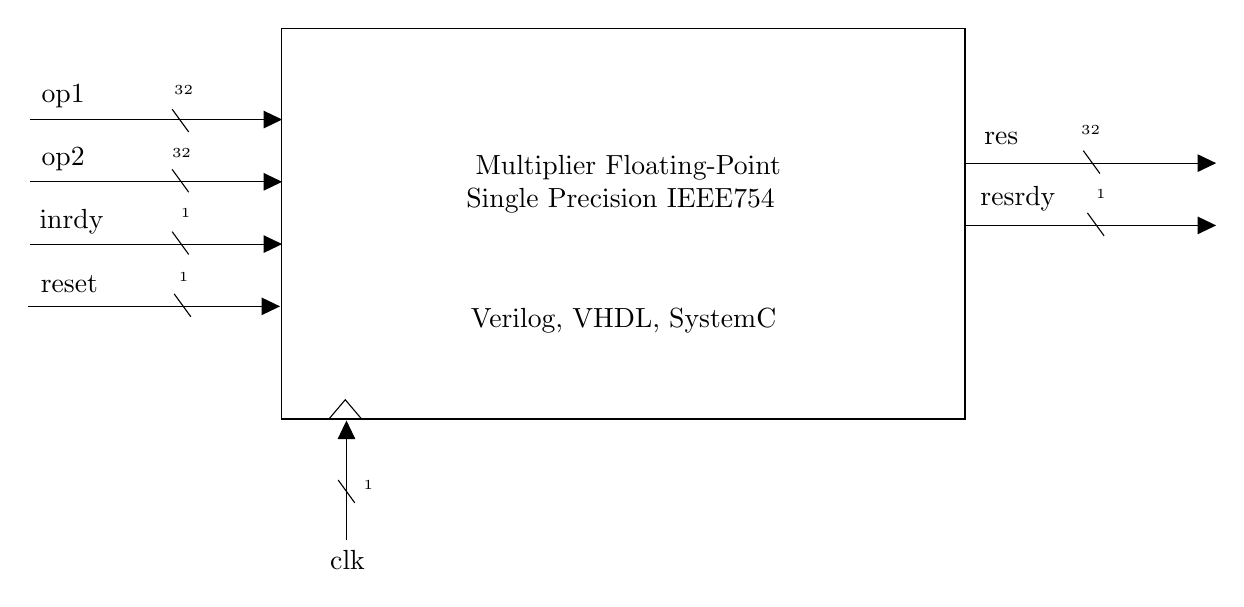
\begin{tikzpicture}[x=0.75pt,y=0.75pt,yscale=-1,xscale=1]
	%uncomment if require: \path (0,406); %set diagram left start at 0, and has height of 406
	
	%Shape: Rectangle [id:dp9211023518838333] 
	\draw   (165,86) -- (494.5,86) -- (494.5,274.29) -- (165,274.29) -- cycle ;
	%Straight Lines [id:da9591337699307748] 
	\draw    (44.17,130) -- (162.5,130) ;
	\draw [shift={(165.5,130)}, rotate = 180] [fill={rgb, 255:red, 0; green, 0; blue, 0 }  ][line width=0.08]  [draw opacity=0] (8.93,-4.29) -- (0,0) -- (8.93,4.29) -- cycle    ;
	
	%Straight Lines [id:da579702478769955] 
	\draw    (44.17,160) -- (162.5,160) ;
	\draw [shift={(165.5,160)}, rotate = 180] [fill={rgb, 255:red, 0; green, 0; blue, 0 }  ][line width=0.08]  [draw opacity=0] (8.93,-4.29) -- (0,0) -- (8.93,4.29) -- cycle    ;
	
	%Straight Lines [id:da76113659482319] 
	\draw    (44.17,190) -- (162.5,190) ;
	\draw [shift={(165.5,190)}, rotate = 180] [fill={rgb, 255:red, 0; green, 0; blue, 0 }  ][line width=0.08]  [draw opacity=0] (8.93,-4.29) -- (0,0) -- (8.93,4.29) -- cycle    ;
	
	%Straight Lines [id:da45600723803220433] 
	\draw    (43.17,220) -- (161.5,220) ;
	\draw [shift={(164.5,220)}, rotate = 180] [fill={rgb, 255:red, 0; green, 0; blue, 0 }  ][line width=0.08]  [draw opacity=0] (8.93,-4.29) -- (0,0) -- (8.93,4.29) -- cycle    ;
	
	%Straight Lines [id:da9181879524908487] 
	\draw    (494.17,151) -- (612.5,151) ;
	\draw [shift={(615.5,151)}, rotate = 180] [fill={rgb, 255:red, 0; green, 0; blue, 0 }  ][line width=0.08]  [draw opacity=0] (8.93,-4.29) -- (0,0) -- (8.93,4.29) -- cycle    ;
	
	%Straight Lines [id:da7910328097566827] 
	\draw    (494.17,181) -- (612.5,181) ;
	\draw [shift={(615.5,181)}, rotate = 180] [fill={rgb, 255:red, 0; green, 0; blue, 0 }  ][line width=0.08]  [draw opacity=0] (8.93,-4.29) -- (0,0) -- (8.93,4.29) -- cycle    ;
	
	%Shape: Triangle [id:dp124533916535147] 
	\draw   (195.92,265) -- (203.83,274.33) -- (188,274.33) -- cycle ;
	%Straight Lines [id:da309296107434495] 
	\draw    (196.5,332.33) -- (196.5,278) ;
	\draw [shift={(196.5,275)}, rotate = 450] [fill={rgb, 255:red, 0; green, 0; blue, 0 }  ][line width=0.08]  [draw opacity=0] (8.93,-4.29) -- (0,0) -- (8.93,4.29) -- cycle    ;
	
	%Straight Lines [id:da1421875224201805] 
	\draw    (112.5,125) -- (120.5,136) ;
	
	
	%Straight Lines [id:da13538438410660247] 
	\draw    (112.5,154) -- (120.5,165) ;
	
	
	%Straight Lines [id:da5317963116700639] 
	\draw    (112.5,184) -- (120.5,195) ;
	
	
	%Straight Lines [id:da8132393230886649] 
	\draw    (113.5,214) -- (121.5,225) ;
	
	
	%Straight Lines [id:da7586641121884944] 
	\draw    (192.5,303.67) -- (200.5,314.67) ;
	
	
	%Straight Lines [id:da33268972261161966] 
	\draw    (551.5,145) -- (559.5,156) ;
	
	
	%Straight Lines [id:da15050698861885248] 
	\draw    (553.5,175) -- (561.5,186) ;
	
	
	
	% Text Node
	\draw (330,161) node   [align=left] { \ Multiplier Floating-Point \\Single Precision IEEE754};
	% Text Node
	\draw (330,227) node   [align=left] {Verilog, VHDL, SystemC};
	% Text Node
	\draw (60,119) node   [align=left] {op1};
	% Text Node
	\draw (60,149) node   [align=left] {op2};
	% Text Node
	\draw (64,179) node   [align=left] {inrdy};
	% Text Node
	\draw (63,209) node   [align=left] {reset};
	% Text Node
	\draw (197,342) node   [align=left] {clk};
	% Text Node
	\draw (512,139) node   [align=left] {res};
	% Text Node
	\draw (520,168) node   [align=left] {resrdy};
	% Text Node
	\draw (555,135) node   [align=left] {{\tiny 32}};
	% Text Node
	\draw (560,166) node   [align=left] {{\tiny 1}};
	% Text Node
	\draw (207,306) node   [align=left] {{\tiny 1}};
	% Text Node
	\draw (118,206) node   [align=left] {{\tiny 1}};
	% Text Node
	\draw (119,175) node   [align=left] {{\tiny 1}};
	% Text Node
	\draw (117,146) node   [align=left] {{\tiny 32}};
	% Text Node
	\draw (118,116) node   [align=left] {{\tiny 32}};
	
		\end{tikzpicture}
			\caption{Multiplier interface schema}
			\label{fig:mul_ieee_754_schema}
		\end{figure*}
	
		\newpage
	\begin{figure*}[t]
		\centering
		
\tikzset{
	->, % makes the edges directed
	>=stealth, % makes the arrow heads bold
	node distance=3.5cm, % specifies the minimum distance between two nodes. Change if n every state/.style={thick, fill=gray!10}, % sets the properties for each ’state’ n initial text=$ $, % sets the text that appears on the start arrow
	font={\fontsize{6pt}{6}\selectfont}
}

		\centering % centers the figure
		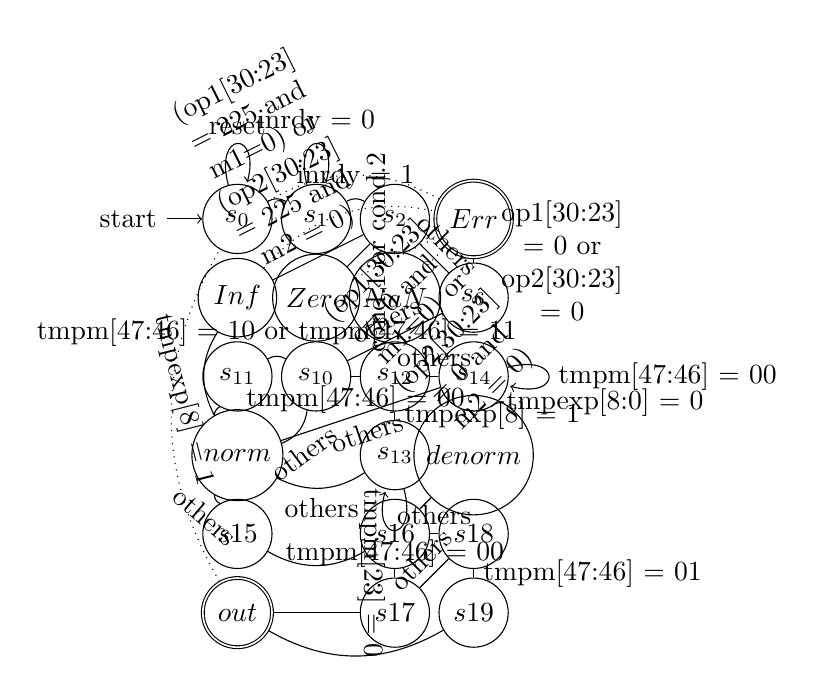
\begin{tikzpicture}
		
		%s0
		\node[state, initial, xshift=-3cm] (s0) {$s_0$};		
		%s1										
		\node[state, right of=s0] (s1) {$s_1$};	
		%s2									
		\node[state, right of=s1] (s2) {$s_2$};		
		%nan								
		\node[state, below of=s2] (NaN) {$NaN$};
		%zero			
		\node[state, below of=s1] (zero) {$Zero$};			
		%inf							
		\node[state, below of=s0] (inf) {$Inf$};
		%s6
		\node[state, right of=NaN] (s6) {$s_6$};
		%err
		\node[state, right of=s2, accepting] (err) {$Err$};
		%s10
		\node[state, below of=zero] (s10) {$s_{10}$};
		%s12
		\node[state, below of=NaN] (s12) {$s_{12}$};
		%s11
		\node[state, below of=inf] (s11) {$s_{11}$};
		%s13
		\node[state, below of=s12] (s13) {$s_{13}$};
		%s14
		\node[state, below of=s6] (s14) {$s_{14}$};
		%norm
		\node[state, below of=s11] (norm) {$norm$};
		%denorm
		\node[state, below of=s14] (denorm) {$denorm$};
		%15
		\node[state, below of=norm] (s15) {$s15$};
		%16
		\node[state, below of=s13] (s16) {$s16$};
		%17
		\node[state, below of=s16] (s17) {$s17$};
		%18
		\node[state, below of=denorm] (s18) {$s18$};
		%19
		\node[state, below of=s18] (s19) {$s19$};
		%out
		\node[state, accepting, below of=s15] (out) {$out$};
		
		
		% S0
		\draw (s0) edge[loop above] node{reset} (s0);
		\draw (s0) edge[bend left, above] node{} (s1);
		
		% S1
		\draw (s1) edge[loop above]  node{inrdy = 0} (s1);
		\draw (s1) edge[bend left, above] node{inrdy = 1} (s2);
		
		% S2
		% cond1: op1(30 DOWNTO 23) = 255 AND m1 /= 0) OR (op2(30 DOWNTO 23) = 255 AND m2 /= 0
		% cond2: (op1(30 DOWNTO 23) = 255 AND m1 = 0 AND op2(30 DOWNTO 23) = 0 AND m2 = 0) OR (op2(30 DOWNTO 23) = 255 AND m2 = 0 AND op1(30 DOWNTO 23) = 0 AND m1 = 0)
		% cond3: op1(30 DOWNTO 23) = 0 AND m1 = 0) OR (op2(30 DOWNTO 23) = 0 AND m2 = 0
		% cond4: op1(30 DOWNTO 23) = 255 AND m1 = 0) OR (op2(30 DOWNTO 23) = 255 AND m2 = 0
		\draw (s2) edge[sloped, above] node{cond.1 or cond.2} (NaN);
		\draw (s2) edge[sloped, below] node[text width=2cm,align=center] {(op1[30:23] = 0 and m1=0) or (op2[30:23] = 0 and m2 = 0)} (zero);
		\draw (s2) edge[sloped, above,] node[text width=2cm,align=center] {(op1[30:23] = 225 and m1=0) or (op2[30:23] = 225 and m2 = 0)} (inf);
		\draw (s2) edge[sloped, above] node{others} (s6);
		
		% S6
		% cond5: (op1(30 DOWNTO 23) = 0 Or op2(30 DOWNTO 23) = 0)
		\draw (s6) edge[below, right] node[text width=2cm,align=center] {op1[30:23] = 0 or op2[30:23] = 0} (err);
		\draw (s6) edge[sloped, above] node{others} (s10);
		
		%s10
		%cond8: (tmpm(47 DOWNTO 46) = "10") OR (tmpm(47 DOWNTO 46) = "11")
		%cond9: (tmpm(47 DOWNTO 46) = "00")
		\draw (s10) edge[above, bend right, sloped]	 node{tmpm[47:46] = 10 or tmpm[47:46] = 11} (s11);
		\draw (s10) edge[below] node{tmpm[47:46] = 00} (s12);
		\draw (s10) edge[near end,bend left, below, sloped] node{others} (norm);
		
		%s11
		\draw (s11) edge[bend right, below] node{} (norm);
		
		%12
		% cond10: tmpexp(8) = 1
		\draw (s12) edge[right] node{tmpexp[8] = 1} (s13);
		\draw (s12) edge[sloped, above] node{others} (s14);
		
		%13
		%cond11:(tmpm(47 DOWNTO 46) = "00")
		\draw (s13) edge[loop below, below] node{tmpm[47:46] = 00} (s13);
		\draw (s13) edge[bend left, below] node{others} (norm);
		
		%14
		%cond12:(tmpm(47 DOWNTO 46) = "00")
		% cond13:(tmpexp(8 DOWNTO 0) = 0)
		\draw (s14) edge[loop right, right] node{tmpm[47:46] = 00} (s14);
		\draw (s14) edge[bend left, above, right] node{tmpexp[8:0] = 0} (denorm);
		\draw (s14) edge[below, sloped] node{others} (norm);
		
		%norm
		%cond14:(tmpexp(8) = '1') 
		\draw (norm) edge[below, bend left, near start, sloped] node{tmpexp[8] = 1} (inf);
		\draw (norm) edge[below, bend right, near end, sloped] node{others} (s15);
		
		%denorm
		\draw (denorm) edge[above] node{} (s16);
		
		%15
		\draw (s15) edge[bend right] node{} (s16);
		
		%16
		%cond15:(tmpm(23) = '0')
		\draw (s16) edge[below, sloped] node{tmpm[23] = 0} (s17);
		\draw (s16) edge[above] node{others} (s18);
		
		%17
		\draw (s17) edge[] node{} (out);
		
		%18
		%cond16:(tmpm(47 DOWNTO 46) = "01")
		\draw (s18) edge[right] node{tmpm[47:46] = 01} (s19);
		\draw (s18) edge[above, sloped] node{others} (s17);
		
		%19
		\draw (s19) edge[above, bend left] node{} (out);
		
		% nan
		\draw[dotted] (NaN) edge[] node{} (err);
		
		%zero
		\draw[dotted] (zero) edge[] node{} (err);
		
		%inf
		\draw[dotted] (inf) edge[bend left] node{} (err);
		
		%out
		\draw[dotted] (out) edge[bend left] node{} (s0);
		
		%err
		\draw[dotted] (err) edge[bend right] node{} (s0);
		
		\end{tikzpicture}
		\caption{EFSM multiplier. The state operation are described on Table~\ref{fig:operationefsm}}
		\label{fig:efsm_mul}
	\end{figure*}

		\newpage
\begin{figure*}[t]
	\centering
	\tikzset{every picture/.style={line width=0.75pt}} %set default line width to 0.75pt        

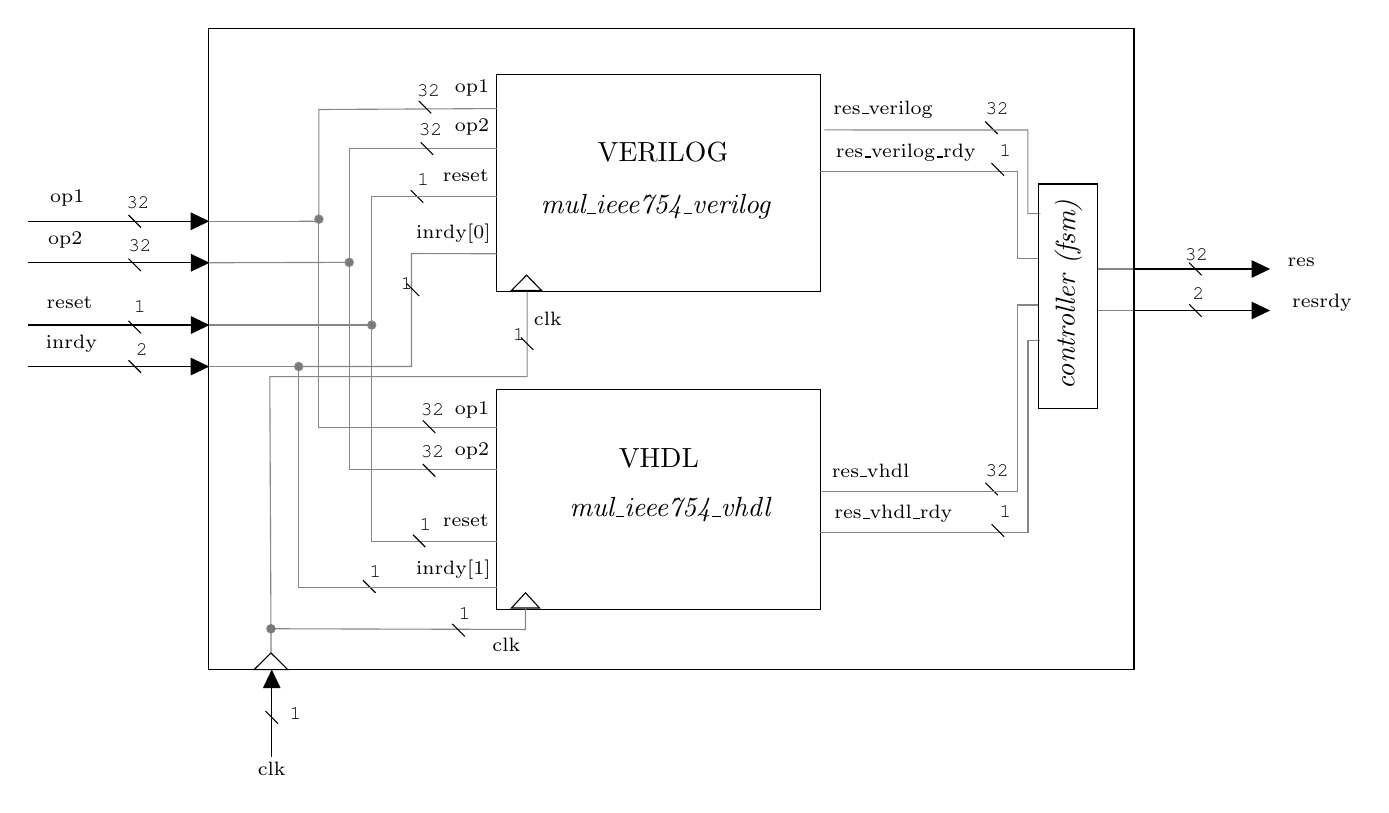
\begin{tikzpicture}[x=0.75pt,y=0.75pt,yscale=-1,xscale=1]
%uncomment if require: \path (0,406); %set diagram left start at 0, and has height of 406

%Shape: Rectangle [id:dp6336663527405302] 
\draw   (107.07,11) -- (552.93,11) -- (552.93,320.02) -- (107.07,320.02) -- cycle ;
%Shape: Triangle [id:dp3281881008560862] 
\draw   (137.12,312) -- (145.24,320.02) -- (129,320.02) -- cycle ;
%Straight Lines [id:da439133343118816] 
\draw    (20.17,104) -- (104.39,104) ;
\draw [shift={(107.39,104)}, rotate = 180] [fill={rgb, 255:red, 0; green, 0; blue, 0 }  ][line width=0.08]  [draw opacity=0] (8.93,-4.29) -- (0,0) -- (8.93,4.29) -- cycle    ;

%Straight Lines [id:da2843684939096296] 
\draw    (20.17,124) -- (104.5,124) ;
\draw [shift={(107.5,124)}, rotate = 180] [fill={rgb, 255:red, 0; green, 0; blue, 0 }  ][line width=0.08]  [draw opacity=0] (8.93,-4.29) -- (0,0) -- (8.93,4.29) -- cycle    ;

%Straight Lines [id:da6753071619116936] 
\draw    (20.17,154) -- (104.5,154) ;
\draw [shift={(107.5,154)}, rotate = 180] [fill={rgb, 255:red, 0; green, 0; blue, 0 }  ][line width=0.08]  [draw opacity=0] (8.93,-4.29) -- (0,0) -- (8.93,4.29) -- cycle    ;

%Straight Lines [id:da20256285976533528] 
\draw    (20.17,174) -- (104.39,174) ;
\draw [shift={(107.39,174)}, rotate = 180] [fill={rgb, 255:red, 0; green, 0; blue, 0 }  ][line width=0.08]  [draw opacity=0] (8.93,-4.29) -- (0,0) -- (8.93,4.29) -- cycle    ;

%Straight Lines [id:da27675265454582976] 
\draw    (68.5,171) -- (74.5,177) ;


%Straight Lines [id:da1848780154326044] 
\draw    (68.5,152) -- (74.5,158) ;


%Straight Lines [id:da03355398321313008] 
\draw    (68.5,122) -- (74.5,128) ;


%Straight Lines [id:da24295909025104223] 
\draw    (68.5,101) -- (74.5,107) ;


%Straight Lines [id:da7767537781347004] 
\draw    (137.5,362) -- (137.5,323) ;
\draw [shift={(137.5,320)}, rotate = 450] [fill={rgb, 255:red, 0; green, 0; blue, 0 }  ][line width=0.08]  [draw opacity=0] (8.93,-4.29) -- (0,0) -- (8.93,4.29) -- cycle    ;

%Straight Lines [id:da9782975999205276] 
\draw    (134.5,340) -- (140.5,346) ;


%Straight Lines [id:da23980175180630126] 
\draw    (552.5,127) -- (615.5,127) ;
\draw [shift={(618.5,127)}, rotate = 180] [fill={rgb, 255:red, 0; green, 0; blue, 0 }  ][line width=0.08]  [draw opacity=0] (8.93,-4.29) -- (0,0) -- (8.93,4.29) -- cycle    ;

%Straight Lines [id:da35605141442667354] 
\draw    (552.5,147) -- (615.5,147) ;
\draw [shift={(618.5,147)}, rotate = 180] [fill={rgb, 255:red, 0; green, 0; blue, 0 }  ][line width=0.08]  [draw opacity=0] (8.93,-4.29) -- (0,0) -- (8.93,4.29) -- cycle    ;

%Straight Lines [id:da2135828501927669] 
\draw    (579.5,144) -- (585.5,150) ;


%Straight Lines [id:da11032934107937131] 
\draw    (579.5,124) -- (585.5,130) ;


%Shape: Rectangle [id:dp6853151840169605] 
\draw   (245.93,33.12) -- (401.99,33.12) -- (401.99,137.8) -- (245.93,137.8) -- cycle ;
%Shape: Rectangle [id:dp7626984189620242] 
\draw   (245.91,185) -- (401.99,185) -- (401.99,290.92) -- (245.91,290.92) -- cycle ;
%Straight Lines [id:da12162208455268808] 
\draw [color={rgb, 255:red, 134; green, 134; blue, 134 }  ,draw opacity=1 ]   (107.39,104) -- (150.5,104) ;


%Straight Lines [id:da8124965754602955] 
\draw [color={rgb, 255:red, 134; green, 134; blue, 134 }  ,draw opacity=1 ]   (107.5,124) -- (174.81,123.81) ;


%Straight Lines [id:da43526973548150383] 
\draw [color={rgb, 255:red, 134; green, 134; blue, 134 }  ,draw opacity=1 ]   (107.5,154) -- (185.67,154) ;


%Straight Lines [id:da022563600394316374] 
\draw [color={rgb, 255:red, 134; green, 134; blue, 134 }  ,draw opacity=1 ]   (107.39,174) -- (150.5,174) ;


%Straight Lines [id:da3226593047060001] 
\draw [color={rgb, 255:red, 134; green, 134; blue, 134 }  ,draw opacity=1 ]   (160.21,105) -- (160.21,203.16) -- (246.21,203.16) ;


%Straight Lines [id:da9727551695527996] 
\draw [color={rgb, 255:red, 134; green, 134; blue, 134 }  ,draw opacity=1 ]   (150.5,104) -- (160.21,104) -- (160.21,50.16) -- (246.18,49.71) ;


%Straight Lines [id:da6367832519772582] 
\draw    (208.31,46) -- (214.31,52) ;


%Straight Lines [id:da46209026866946745] 
\draw    (204.5,89) -- (210.5,95) ;


%Straight Lines [id:da8905265773131018] 
\draw    (181.5,277) -- (187.5,283) ;


%Straight Lines [id:da5019563800088057] 
\draw    (210.31,200) -- (216.31,206) ;


%Straight Lines [id:da1033499993584861] 
\draw [color={rgb, 255:red, 134; green, 134; blue, 134 }  ,draw opacity=1 ]   (174.81,125.81) -- (174.81,223.81) -- (245.82,223.81) ;


%Straight Lines [id:da5009224027009053] 
\draw    (210.31,221) -- (216.31,227) ;


%Straight Lines [id:da8027396524130416] 
\draw [color={rgb, 255:red, 134; green, 134; blue, 134 }  ,draw opacity=1 ]   (174.81,123.81) -- (174.81,68.81) -- (245.82,68.81) ;


%Straight Lines [id:da40409487095596963] 
\draw    (209.31,66) -- (215.31,72) ;


%Straight Lines [id:da5607632824061252] 
\draw [color={rgb, 255:red, 134; green, 134; blue, 134 }  ,draw opacity=1 ]   (185.67,154) -- (185.67,92.01) -- (245.82,92.01) ;


%Straight Lines [id:da5283862800462044] 
\draw [color={rgb, 255:red, 134; green, 134; blue, 134 }  ,draw opacity=1 ]   (185.67,156) -- (185.67,258.33) -- (245.82,258.33) ;


%Straight Lines [id:da7508526443917787] 
\draw    (205.5,255) -- (211.5,261) ;


%Straight Lines [id:da20759705658555372] 
\draw [color={rgb, 255:red, 134; green, 134; blue, 134 }  ,draw opacity=1 ]   (150.5,176) -- (150.5,280.48) -- (246.13,280.48) ;


%Straight Lines [id:da03284102275954337] 
\draw [color={rgb, 255:red, 134; green, 134; blue, 134 }  ,draw opacity=1 ]   (150.5,174) -- (204.82,174) -- (204.82,119.54) -- (245.83,119.67) ;


%Straight Lines [id:da8811556435028376] 
\draw    (202.5,134) -- (208.5,140) ;


%Shape: Circle [id:dp6702960483681197] 
\draw  [color={rgb, 255:red, 134; green, 134; blue, 134 }  ,draw opacity=1 ][fill={rgb, 255:red, 122; green, 121; blue, 121 }  ,fill opacity=1 ] (158.21,103) .. controls (158.21,101.9) and (159.11,101) .. (160.21,101) .. controls (161.32,101) and (162.21,101.9) .. (162.21,103) .. controls (162.21,104.1) and (161.32,105) .. (160.21,105) .. controls (159.11,105) and (158.21,104.1) .. (158.21,103) -- cycle ;
%Shape: Circle [id:dp03857221501315067] 
\draw  [color={rgb, 255:red, 134; green, 134; blue, 134 }  ,draw opacity=1 ][fill={rgb, 255:red, 122; green, 121; blue, 121 }  ,fill opacity=1 ] (172.81,123.81) .. controls (172.81,122.7) and (173.71,121.81) .. (174.81,121.81) .. controls (175.92,121.81) and (176.81,122.7) .. (176.81,123.81) .. controls (176.81,124.91) and (175.92,125.81) .. (174.81,125.81) .. controls (173.71,125.81) and (172.81,124.91) .. (172.81,123.81) -- cycle ;
%Shape: Circle [id:dp5204851935389241] 
\draw  [color={rgb, 255:red, 134; green, 134; blue, 134 }  ,draw opacity=1 ][fill={rgb, 255:red, 122; green, 121; blue, 121 }  ,fill opacity=1 ] (183.67,154) .. controls (183.67,152.9) and (184.56,152) .. (185.67,152) .. controls (186.77,152) and (187.67,152.9) .. (187.67,154) .. controls (187.67,155.1) and (186.77,156) .. (185.67,156) .. controls (184.56,156) and (183.67,155.1) .. (183.67,154) -- cycle ;
%Shape: Circle [id:dp3844621887429003] 
\draw  [color={rgb, 255:red, 134; green, 134; blue, 134 }  ,draw opacity=1 ][fill={rgb, 255:red, 122; green, 121; blue, 121 }  ,fill opacity=1 ] (148.5,174) .. controls (148.5,172.9) and (149.4,172) .. (150.5,172) .. controls (151.6,172) and (152.5,172.9) .. (152.5,174) .. controls (152.5,175.1) and (151.6,176) .. (150.5,176) .. controls (149.4,176) and (148.5,175.1) .. (148.5,174) -- cycle ;
%Shape: Triangle [id:dp8339553439830822] 
\draw   (259.75,283) -- (266.5,290.33) -- (253,290.33) -- cycle ;
%Shape: Triangle [id:dp9846003194523182] 
\draw   (260.25,130) -- (267.5,137.33) -- (253,137.33) -- cycle ;
%Straight Lines [id:da7421583912516101] 
\draw [color={rgb, 255:red, 134; green, 134; blue, 134 }  ,draw opacity=1 ]   (137.12,312) -- (137.12,300.33) -- (259.75,300.67) -- (259.75,290.67) ;


%Straight Lines [id:da5799463307833818] 
\draw    (224.5,298) -- (230.5,304) ;


%Straight Lines [id:da5702045435076585] 
\draw [color={rgb, 255:red, 134; green, 134; blue, 134 }  ,draw opacity=1 ]   (137.12,301.33) -- (136.56,178.89) -- (260.56,178.89) -- (260.56,137.89) ;


%Shape: Circle [id:dp3378787613167842] 
\draw  [color={rgb, 255:red, 122; green, 121; blue, 121 }  ,draw opacity=1 ][fill={rgb, 255:red, 122; green, 121; blue, 121 }  ,fill opacity=1 ] (135.12,300.33) .. controls (135.12,299.23) and (136.02,298.33) .. (137.12,298.33) .. controls (138.23,298.33) and (139.12,299.23) .. (139.12,300.33) .. controls (139.12,301.44) and (138.23,302.33) .. (137.12,302.33) .. controls (136.02,302.33) and (135.12,301.44) .. (135.12,300.33) -- cycle ;
%Straight Lines [id:da7002757308564248] 
\draw    (257.5,160) -- (263.5,166) ;


%Straight Lines [id:da3078009528954999] 
\draw    (481.31,56) -- (487.31,62) ;


%Straight Lines [id:da06782591985654118] 
\draw [color={rgb, 255:red, 134; green, 134; blue, 134 }  ,draw opacity=1 ]   (403.76,60) -- (501.77,60.06) -- (501.77,100.33) -- (507.83,100.33) ;


%Straight Lines [id:da2601529714736176] 
\draw [color={rgb, 255:red, 134; green, 134; blue, 134 }  ,draw opacity=1 ]   (401.76,80) -- (496.77,80) -- (496.77,122.06) -- (506.77,122.06) ;


%Straight Lines [id:da06282979955060941] 
\draw    (484.31,76) -- (490.31,82) ;


%Straight Lines [id:da44023450926126706] 
\draw    (481.31,230) -- (487.31,236) ;


%Straight Lines [id:da5028973988120796] 
\draw [color={rgb, 255:red, 134; green, 134; blue, 134 }  ,draw opacity=1 ]   (402.76,234) -- (496.83,234) -- (496.83,144.33) -- (506.83,144.33) ;


%Straight Lines [id:da9272786493811391] 
\draw [color={rgb, 255:red, 134; green, 134; blue, 134 }  ,draw opacity=1 ]   (401.76,254) -- (501.83,254) -- (501.83,161.33) -- (507.83,161.33) ;


%Straight Lines [id:da9957982211718097] 
\draw    (484.31,250) -- (490.31,256) ;


%Shape: Rectangle [id:dp917001202256437] 
\draw   (506.91,86.06) -- (535.31,86.06) -- (535.31,194.06) -- (506.91,194.06) -- cycle ;
%Straight Lines [id:da5355241097155387] 
\draw [color={rgb, 255:red, 134; green, 134; blue, 134 }  ,draw opacity=1 ]   (535.77,147) -- (552.5,147) ;


%Straight Lines [id:da5675288668644215] 
\draw [color={rgb, 255:red, 134; green, 134; blue, 134 }  ,draw opacity=1 ]   (535.77,127) -- (552.5,127) ;



% Text Node
\draw (39,93) node  [font=\normalsize] [align=left] {{\scriptsize op1}};
% Text Node
\draw (38,113) node  [font=\normalsize] [align=left] {{\scriptsize op2}};
% Text Node
\draw (40,143) node  [font=\normalsize] [align=left] {{\scriptsize reset}};
% Text Node
\draw (41,163) node  [font=\normalsize] [align=left] {{\scriptsize inrdy}};
% Text Node
\draw (137.5,368) node   [align=left] {{\scriptsize clk}};
% Text Node
\draw (633.5,124) node   [align=left] {{\scriptsize res}};
% Text Node
\draw (643.5,143) node   [align=left] {{\scriptsize resrdy}};
% Text Node
\draw (73,95) node  [font=\tiny] [align=left] {{\scriptsize {\fontfamily{pcr}\selectfont 32}}};
% Text Node
\draw (74,116) node  [font=\tiny] [align=left] {{\scriptsize {\fontfamily{pcr}\selectfont 32}}};
% Text Node
\draw (74,145) node  [font=\tiny] [align=left] {{\scriptsize {\fontfamily{pcr}\selectfont 1}}};
% Text Node
\draw (75,166) node  [font=\tiny] [align=left] {{\scriptsize {\fontfamily{pcr}\selectfont 2}}};
% Text Node
\draw (149,341) node  [font=\tiny] [align=left] {{\scriptsize {\fontfamily{pcr}\selectfont 1}}};
% Text Node
\draw (583,120) node  [font=\tiny] [align=left] {{\scriptsize {\fontfamily{pcr}\selectfont 32}}};
% Text Node
\draw (584,139) node  [font=\tiny] [align=left] {{\scriptsize {\fontfamily{pcr}\selectfont 2}}};
% Text Node
\draw (324,218) node   [align=left] {VHDL};
% Text Node
\draw (326,70.46) node   [align=left] {VERILOG};
% Text Node
\draw (234,40) node   [align=left] {{\scriptsize op1}};
% Text Node
\draw (234,58.5) node   [align=left] {{\scriptsize op2}};
% Text Node
\draw (234,195) node   [align=left] {{\scriptsize op1}};
% Text Node
\draw (231,248) node   [align=left] {{\scriptsize reset}};
% Text Node
\draw (213,41) node  [font=\tiny] [align=left] {{\scriptsize {\fontfamily{pcr}\selectfont 32}}};
% Text Node
\draw (210.5,84) node  [font=\tiny] [align=left] {{\scriptsize {\fontfamily{pcr}\selectfont 1}}};
% Text Node
\draw (187.5,273) node  [font=\tiny] [align=left] {{\scriptsize {\fontfamily{pcr}\selectfont 1}}};
% Text Node
\draw (330,243) node   [align=left] {\textit{mul\_ieee754\_vhdl}};
% Text Node
\draw (323,97) node   [align=left] {\textit{mul\_ieee754\_verilog}};
% Text Node
\draw (215,195) node  [font=\tiny] [align=left] {{\scriptsize {\fontfamily{pcr}\selectfont 32}}};
% Text Node
\draw (215,215) node  [font=\tiny] [align=left] {{\scriptsize {\fontfamily{pcr}\selectfont 32}}};
% Text Node
\draw (234,215) node   [align=left] {{\scriptsize op2}};
% Text Node
\draw (214,60) node  [font=\tiny] [align=left] {{\scriptsize {\fontfamily{pcr}\selectfont 32}}};
% Text Node
\draw (231,82) node   [align=left] {{\scriptsize reset}};
% Text Node
\draw (211.5,250) node  [font=\tiny] [align=left] {{\scriptsize {\fontfamily{pcr}\selectfont 1}}};
% Text Node
\draw (225,272) node   [align=left] {{\scriptsize inrdy[1]}};
% Text Node
\draw (225,110) node   [align=left] {{\scriptsize inrdy[0]}};
% Text Node
\draw (202.5,134) node  [font=\tiny] [align=left] {{\scriptsize {\fontfamily{pcr}\selectfont 1}}};
% Text Node
\draw (250.5,308) node   [align=left] {{\scriptsize clk}};
% Text Node
\draw (230.5,293) node  [font=\tiny] [align=left] {{\scriptsize {\fontfamily{pcr}\selectfont 1}}};
% Text Node
\draw (270.5,151) node   [align=left] {{\scriptsize clk}};
% Text Node
\draw (256.56,158.39) node  [font=\tiny] [align=left] {{\scriptsize {\fontfamily{pcr}\selectfont 1}}};
% Text Node
\draw (487,50) node  [font=\tiny] [align=left] {{\scriptsize {\fontfamily{pcr}\selectfont 32}}};
% Text Node
\draw (432,50) node   [align=left] {{\scriptsize res\_verilog}};
% Text Node
\draw (443,71) node   [align=left] {{\scriptsize res\_verilog\_rdy}};
% Text Node
\draw (491,70) node  [font=\tiny] [align=left] {{\scriptsize {\fontfamily{pcr}\selectfont 1}}};
% Text Node
\draw (487,224) node  [font=\tiny] [align=left] {{\scriptsize {\fontfamily{pcr}\selectfont 32}}};
% Text Node
\draw (426,224) node   [align=left] {{\scriptsize res\_vhdl}};
% Text Node
\draw (437,245) node   [align=left] {{\scriptsize res\_vhdl\_rdy}};
% Text Node
\draw (491,244) node  [font=\tiny] [align=left] {{\scriptsize {\fontfamily{pcr}\selectfont 1}}};
% Text Node
\draw (521.11,139.06) node  [rotate=-270.28] [align=left] {\textit{controller (fsm)}};


\end{tikzpicture}

	\caption{Toplevel interface schema}
	\label{fig:tl}
\end{figure*}


\begin{figure*}[t]
	\centering
	
\tikzset{
	->, % makes the edges directed
	>=stealth, % makes the arrow heads bold
	node distance=5cm, % specifies the minimum distance between two nodes. Change if n every state/.style={thick, fill=gray!10}, % sets the properties for each ’state’ n initial text=$ $, % sets the text that appears on the start arrow
}

		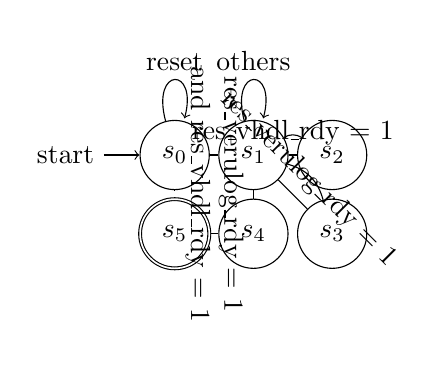
\begin{tikzpicture}
		
		%s0
		\node[state, initial] (s0) {$s_0$};		
		%s1										
		\node[state, right of=s0] (s1) {$s_1$};	
		%s2									
		\node[state, right of=s1] (s2) {$s_2$};		
		%s3								
		\node[state, below of=s2] (s3) {$s_3$};
		%s4			
		\node[state, below of=s1] (s4) {$s_4$};			
		%s5							
		\node[state, below of=s0, accepting] (s5) {$s_5$};
		
		
		\draw (s0) edge[loop above] node{reset} (s0);
		\draw (s0) edge[above] node{} (s1);
		\draw (s1) edge[above, sloped] node{res\_vhdl\_rdy = 1} (s2);
		\draw (s1) edge[loop above, sloped] node{others} (s1);
		\draw (s1) edge[above, sloped] node{res\_verulog\_rdy = 1} (s3);
		\draw (s1) edge[below, sloped] node[text width=4cm,align=center]  {res\_verulog\_rdy = 1 and res\_vhdl\_rdy = 1} (s4);
		\draw (s2) edge[above, bend right] node{} (s1);
		\draw (s3) edge[above, bend right] node{} (s1);
		\draw (s4) edge[above] (s5);
		\draw[dotted] (s5) edge[above] (s0);
		
		
		\end{tikzpicture}
	\caption{EFSM toplevel}
	\label{fig:efsm_tl}
\end{figure*}


\begin{figure*}[t]
	\centering
	
	\tikzset{every picture/.style={line width=0.75pt}} %set default line width to 0.75pt        
	
	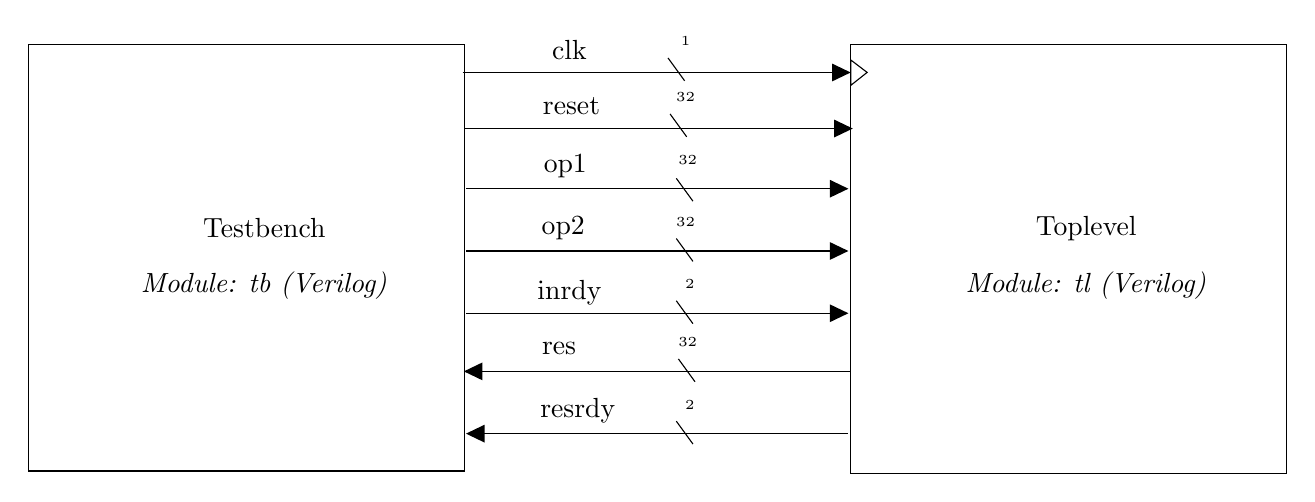
\begin{tikzpicture}[x=0.75pt,y=0.75pt,yscale=-1,xscale=1]
	%uncomment if require: \path (0,406); %set diagram left start at 0, and has height of 406
	
	%Shape: Rectangle [id:dp9211023518838333] 
	\draw   (28.25,60.54) -- (238.5,60.54) -- (238.5,266) -- (28.25,266) -- cycle ;
	%Straight Lines [id:da9591337699307748] 
	\draw    (239.17,130) -- (420.4,130) ;
	\draw [shift={(423.4,130)}, rotate = 180] [fill={rgb, 255:red, 0; green, 0; blue, 0 }  ][line width=0.08]  [draw opacity=0] (8.93,-4.29) -- (0,0) -- (8.93,4.29) -- cycle    ;
	
	%Straight Lines [id:da579702478769955] 
	\draw    (239.17,160) -- (420.4,160) ;
	\draw [shift={(423.4,160)}, rotate = 180] [fill={rgb, 255:red, 0; green, 0; blue, 0 }  ][line width=0.08]  [draw opacity=0] (8.93,-4.29) -- (0,0) -- (8.93,4.29) -- cycle    ;
	
	%Straight Lines [id:da76113659482319] 
	\draw    (239.17,190) -- (420.4,190) ;
	\draw [shift={(423.4,190)}, rotate = 180] [fill={rgb, 255:red, 0; green, 0; blue, 0 }  ][line width=0.08]  [draw opacity=0] (8.93,-4.29) -- (0,0) -- (8.93,4.29) -- cycle    ;
	
	%Straight Lines [id:da45600723803220433] 
	\draw    (238.5,101) -- (422.5,101) ;
	\draw [shift={(425.5,101)}, rotate = 180] [fill={rgb, 255:red, 0; green, 0; blue, 0 }  ][line width=0.08]  [draw opacity=0] (8.93,-4.29) -- (0,0) -- (8.93,4.29) -- cycle    ;
	
	%Shape: Triangle [id:dp124533916535147] 
	\draw   (432.43,73.96) -- (424.51,67.94) -- (424.63,80.14) -- cycle ;
	%Straight Lines [id:da1421875224201805] 
	\draw    (340.5,125) -- (348.5,136) ;
	
	
	%Straight Lines [id:da13538438410660247] 
	\draw    (340.5,154) -- (348.5,165) ;
	
	
	%Straight Lines [id:da5317963116700639] 
	\draw    (340.5,184) -- (348.5,195) ;
	
	
	%Straight Lines [id:da8132393230886649] 
	\draw    (337.5,94) -- (345.5,105) ;
	
	
	%Shape: Rectangle [id:dp6892399379315668] 
	\draw   (424.25,60.54) -- (634.5,60.54) -- (634.5,267) -- (424.25,267) -- cycle ;
	%Straight Lines [id:da04738946392112342] 
	\draw    (241.14,218) -- (424.5,218) ;
	
	\draw [shift={(238.14,218)}, rotate = 0] [fill={rgb, 255:red, 0; green, 0; blue, 0 }  ][line width=0.08]  [draw opacity=0] (8.93,-4.29) -- (0,0) -- (8.93,4.29) -- cycle    ;
	%Straight Lines [id:da32617397066684783] 
	\draw    (341.5,212) -- (349.5,223) ;
	
	
	%Straight Lines [id:da8691621982326109] 
	\draw    (242.17,248) -- (423.4,248) ;
	
	\draw [shift={(239.17,248)}, rotate = 0] [fill={rgb, 255:red, 0; green, 0; blue, 0 }  ][line width=0.08]  [draw opacity=0] (8.93,-4.29) -- (0,0) -- (8.93,4.29) -- cycle    ;
	%Straight Lines [id:da7911020252616261] 
	\draw    (340.5,242) -- (348.5,253) ;
	
	
	%Straight Lines [id:da25458565339624795] 
	\draw    (237.5,74) -- (421.5,74) ;
	\draw [shift={(424.5,74)}, rotate = 180] [fill={rgb, 255:red, 0; green, 0; blue, 0 }  ][line width=0.08]  [draw opacity=0] (8.93,-4.29) -- (0,0) -- (8.93,4.29) -- cycle    ;
	
	%Straight Lines [id:da27828416860185] 
	\draw    (336.5,67) -- (344.5,78) ;
	
	
	
	% Text Node
	\draw (142,149) node   [align=left] {Testbench};
	% Text Node
	\draw (287,119) node   [align=left] {op1};
	% Text Node
	\draw (286,149) node   [align=left] {op2};
	% Text Node
	\draw (289,180) node   [align=left] {inrdy};
	% Text Node
	\draw (290,90) node   [align=left] {reset};
	% Text Node
	\draw (347,176) node   [align=left] {{\tiny 2}};
	% Text Node
	\draw (345,146) node   [align=left] {{\tiny 32}};
	% Text Node
	\draw (346,116) node   [align=left] {{\tiny 32}};
	% Text Node
	\draw (142,183) node   [align=left] {\textit{Module: tb (Verilog)}\\};
	% Text Node
	\draw (538,149) node   [align=left] {Toplevel};
	% Text Node
	\draw (538,183) node   [align=left] {\textit{Module: tl (Verilog)}\\};
	% Text Node
	\draw (284,207) node   [align=left] {res};
	% Text Node
	\draw (346,204) node   [align=left] {{\tiny 32}};
	% Text Node
	\draw (293,237) node   [align=left] {resrdy};
	% Text Node
	\draw (347,234) node   [align=left] {{\tiny 2}};
	% Text Node
	\draw (289,63) node   [align=left] {clk};
	% Text Node
	\draw (345,59) node   [align=left] {{\tiny 1}};
	% Text Node
	\draw (345,86) node   [align=left] {{\tiny 32}};
	
	
	\end{tikzpicture}
	
	\caption{FSMD testbench}
	\label{fig:fsmd_tb}
\end{figure*}

\begin{figure*}[tb]
	\centering
	\includegraphics[scale=0.40]{figures/vivados1.png}
	\caption{Vivado Simulation Example nr.1 with one input}
	\label{fig:vivado_s1}
\end{figure*}
\begin{figure*}[tb]
	\centering
	\includegraphics[scale=0.38]{figures/vivados2.png}
	\caption{Vivado Simulation Example nr.2 with 10 inputs. The red arrows indicate when the $res$ is outputting the value}
	\label{fig:vivado_s2}
\end{figure*}
\begin{figure*}[tb]
	\centering
	\includegraphics[scale=0.46]{figures/vivados2detail.png}
	\caption{Vivado Simulation Example nr.3, Zoom at the $26,585ns$ of the simulation nr.2 }
	\label{fig:vivado_s2_detail}
\end{figure*}
\begin{figure*}[tb]
\centering
\includegraphics[scale=0.38]{figures/vivados3.png}
\caption{Vivado Simulation Example nr.4, Zoom inside the VHDL multiplier component }
\label{fig:vivado_s3}
\end{figure*}
\begin{figure*}[tb]
	\centering
	\includegraphics[scale=0.38]{figures/vivados4.png}
	\caption{Vivado Simulation Example nr.5, Zoom inside the VHDL multiplier component }
	\label{fig:vivado_s4}
\end{figure*}

	
	
\end{document}